\documentclass[11pt]{article}
\usepackage{tikz}
\usepackage{adjustbox}
\usepackage{amsmath}
\usepackage{tabularx}
\usepackage{float}
\usepackage[brazilian,english]{babel}
\usetikzlibrary{automata,positioning}
\begin{document}



\section*{Primeira Etapa}

\subsection*{Gramática livre de contexto}


$\langle \text{Sofware} \rangle \rightarrow \textbf{programa } \textbf{id} \langle\text{bloco}\rangle$\\\\
$\langle\text{bloco}\rangle \rightarrow \textbf{\{} \langle\text{conteudoBloco}\rangle \textbf{\}}$\\\\
$\langle\text{conteudoBloco}\rangle \rightarrow \langle\text{listaVariaviaveis}\rangle \langle\text{listaComandos}\rangle$\\\\
$\langle\text{listaVariaviaveis}\rangle \rightarrow \langle\text{declaracaoDeVariavel}\rangle \langle\text{listaVariaviaveis}\rangle | \epsilon $\\\\
$\langle\text{listaComandos}\rangle \rightarrow \langle\text{comando}\rangle \langle\text{listaComandos}\rangle | \epsilon $\\\\
$\langle\text{declaracaoDeVariavel}\rangle  \rightarrow \textbf{TipoDeVariavel} \textbf{:} \langle\text{listaIds}\rangle \textbf{;}$\\\\
$\langle\text{comando}\rangle \rightarrow \langle\text{cmdSelecao}\rangle | \langle\text{cmdRepeticaoWhile}\rangle | \langle\text{cmdRepeticaoDoUntil}\rangle | \langle\text{cmdAtribuicao}\rangle$\\\\
$\langle\text{listaIds}\rangle \rightarrow \textbf{id} \langle\text{maisDeUmID} \rangle$\\\\
$\langle\text{maisDeUmID}\rangle \rightarrow \textbf{,}\langle\text{listaIds}\rangle  | \epsilon$\\\\
$\langle\text{cmdSelecao}\rangle \rightarrow \textbf{if(} \langle\text{condicao}\rangle \textbf{)then} \langle\text{bloco}\rangle \langle \text{comElse} \rangle$\\\\
$\langle \text{comElse} \rangle \rightarrow  \textbf{else} \langle\text{bloco}\rangle | \epsilon \\\\$
$\langle\text{cmdRepeticaoWhile}\rangle \rightarrow \textbf{while(} \langle\text{condicao}\rangle \textbf{)} \langle\text{bloco}\rangle $\\\\
$\langle\text{cmdRepeticaoDoUntil}\rangle \rightarrow \textbf{do} \langle\text{bloco}\rangle \textbf{until(} \langle\text{condicao}\rangle \textbf{)} \textbf{;}$\\\\
$\langle\text{cmdAtribuicao}\rangle \rightarrow  \textbf{id} \textbf{:=} \langle\text{expressaoAritmeticaOuConstAscii}\rangle \textbf{;} $\\\\
$\langle\text{condicao}\rangle \rightarrow  \langle\text{idOUConstante}\rangle \textbf{operadorLogico} \langle\text{idOUConstante}\rangle $\\\\%\langle\text{condicao'}\rangle 
% $\langle\text{condicao'}\rangle \rightarrow  \textbf{operadorLogico} \langle\text{condicao}\rangle | \epsilon $\\\\
$\langle\text{idOUConstante}\rangle \rightarrow  \textbf{id }|  \textbf{ ConstInt } | \textbf{ ConstReal } | \textbf{ ConstAscii}$\\\\
$\langle\text{expressaoAritmeticaOuConstAscii}\rangle \rightarrow \langle\text{expressaoAritmetica}\rangle | \textbf{ ConstAscii}$\\\\
$\langle\text{expressaoAritmetica}\rangle \rightarrow  \langle\text{termo}\rangle \langle\text{expressaoAritmetica'}\rangle$\\\\
$\langle\text{expressaoAritmetica'}\rangle \rightarrow \langle\text{addOUsub}\rangle \langle\text{termo}\rangle \langle\text{expressaoAritmetica'}\rangle | \epsilon $\\\\
$\langle\text{termo}\rangle \rightarrow \langle\text{fator}\rangle \langle\text{termo'}\rangle $\\\\
$\langle\text{termo'}\rangle \rightarrow \langle\text{multOUdiv}\rangle \langle\text{fator}\rangle \langle\text{termo'}\rangle | \epsilon $\\\\
$\langle\text{fator}\rangle \rightarrow \textbf{id }| \textbf{ ConstInt } | \textbf{ ConstReal } $\\\\
$\langle\text{addOUsub}\rangle \rightarrow  \textbf{add } | \textbf{ sub}$ \\\\
$\langle\text{multOUdiv}\rangle \rightarrow  \textbf{mult } | \textbf{ div}$ \\\\






\begin{table}[H]
    \hspace{-0.7cm}
    \begin{tabular}{c|c|c}
        \hline
        \textbf{Lexemas}   & \textbf{Nome do Token}   & \textbf{Valor do atributo}  \\
        \hline
         Qualquer ws        &        -                 &            -                \\
        \hline
         programa           &        Programa          &            -                \\
        \hline
         if                &        If                &            -                \\
        \hline
         then              &        Then              &            -                \\
        \hline
         else              &        Else              &            -                \\
        \hline
         while             &        While             &            -                \\
        \hline
         do                &        Do                &            -                \\
        \hline
         until             &        Until             &            -                \\
        \hline
        \hline
         Qualquer ID                          &      Id                   &           posição na tabela \\
        \hline
         numeros inteiros                     &      ConstInt             &          posição na tabela  \\
        \hline
         numeros reais                        &      ConstReal            &          posição na tabela  \\
        \hline
         letras e digitos da tabela ascii     &      ConstAscii           &         posição na tabela   \\
        \hline
        \hline
         ascii             &      TipoDeVariavel      &           Ascii                      \\
        \hline
         int               &      TipoDeVariavel      &           Inteiro                    \\
        \hline
         real              &      TipoDeVariavel      &           Real                       \\
        \hline
        \hline
         ;                 &        PontoTerminação   &            -                \\
        \hline
         ,                 &        Virgula           &            -                \\
        \hline
         :                 &        DoisPontos        &            -                \\
        \hline
         \{                &        AbreChaves        &            -                \\
        \hline
         \}                &        FechaChaves       &            -                \\
        \hline
         (                 &        AbreParênteses    &            -                \\
        \hline
         )                 &        FechaParênteses   &            -                \\
        \hline
        \hline
         $==$              &      OperadorLógico  &            Igual                     \\
        \hline
         $<>$              &      OperadorLógico  &            Diferente                 \\
        \hline
         $<$               &      OperadorLógico  &            Menor                     \\
        \hline
         $>$               &      OperadorLógico  &            Maior                     \\
        \hline
         $<=$              &      OperadorLógico  &            Menor ou igual            \\
        \hline
         $>=$              &      OperadorLógico  &            Maior  ou igual           \\
        \hline
        \hline
         $+$               &      add             &            Soma                      \\
        \hline
         $-$               &      sub             &            Subtração                 \\
        \hline
         $*$               &      mult            &            Multiplicação             \\
        \hline
         $/$               &      div             &            Divisão                   \\
        \hline
        \hline
         $:=$              &      OperadorAtribuição  &            -                         \\
        \hline
       

        
    \end{tabular}
    \caption{Tabela de Tokens}
\end{table}



\begin{table}[H]
    \begin{tabularx}{\textwidth}{c|X}
        \hline
        \textbf{Nome do Token} & \textbf{Expressão regular}   \\ 
        \hline
        programaPrograma & programa  \\  
        \hline
        If  & if \\
        \hline
        Then & then  \\
        \hline
        Else & else \\
        \hline
        While  & while \\
        \hline
        Do & do \\
        \hline
        Until  & until \\
        \hline
        \hline
        PontoTerminação  & ; \\
        \hline
        Virgula  & , \\
        \hline
        DoisPontos  & : \\
        \hline
        AbreChaves  & \{ \\
        \hline
        FechaChaves  & \} \\
        \hline
        AbreParênteses  & ( \\
        \hline
        FechaParênteses  & ) \\
        \hline
        \hline
        OperadorLógico & $<> | == | > | < | <= | >= $   \\
        \hline
        add & $+$   \\
        \hline
        sub & $ - $   \\
        \hline
        mult & $ * $   \\
        \hline
        div & $ / $   \\
        \hline
        \hline
        OperadorAtribuição & := \\
        \hline
        \hline
        TipoDeVariavel & real $|$ ascii $|$ int \\  
        \hline
        \hline
        Id & $(\text{(a..z)}|\text{(A..Z)}|\text{(0..9)})^{+}$ \\
        \hline
        \hline
        ConstInt & ($+ | -| \text{(0..9)}$)(0..9)$^{+}$ \\
        \hline
        ConstReal & (ConstInt.(0..9)$^+$)($((E|e)(+|-)$(0..9)$^+) | \epsilon$)  \\
        \hline
        ConstAscii & '($\text{(a..z)}|\text{(A..Z)}|\text{(0..9)}$)' \\    
        \hline
        [\textit{comentário}] & [[ \^{}]]] \\
        \hline
    \end{tabularx}
    \caption{Token e sua respectiva expressão regular}
\end{table}

\newpage

\section*{Segunda Etapa}


\begin{figure}[H]
    
\end{figure}


% FIRST[SOFTWARE] = programa
% FIRST[BLOCO] = {
% FIRST[CONTEUDOBLOCO] = id TipoDeVariavel if while do
% FIRST[LISTAVARIAVEIS] = TipoDeVariavel
% FIRST[LISTACOMANDOS] = id if while do
% FIRST[DECLARACAODEVARIAVEL] = TipoDeVariavel
% FIRST[COMANDO] = id if while do
% FIRST[LISTAIDS] = id
% FIRST[COMANDOSELECAO] = if
% FIRST[COMANDOREPETICAO] = while do
% FIRST[COMANDOATRIBUICAO] = id
% FIRST[maisDeUmID] = ,
% FIRST[CONDICAO] = id ConstAscii ConstInt ConstReal
% FIRST[COMELSE] = else
% FIRST[CMDREPETICAOWHILE] = while
% FIRST[CMDREPETICAODOUNTIL] = do
% FIRST[EXPRESSAOARITMETICAOUCONSTASCII] = id ConstAscii ConstInt ConstReal
% FIRST[IDOUCONSTATE] = id ConstAscii ConstInt ConstReal
% FIRST[CONDICAO'] = operadorLogico
% FIRST[EXPRESSAOARITMETICA] = id ConstInt ConstReal
% FIRST[TERMO] = id ConstInt ConstReal
% FIRST[EXPRESSAOARITMETICA'] = add sub
% FIRST[ADDOUSUB] = add sub
% FIRST[FATOR] = id ConstInt ConstReal
% FIRST[TERMO'] = mult div
% FIRST[MULTOUDIV] = mult div
% FIRST[CONSTANTE] = ConstAscii ConstInt ConstReal

% FOLLOW[SOFTWARE] =
% FOLLOW[BLOCO] = id $ } if else while do until
% FOLLOW[CONTEUDOBLOCO] = }
% FOLLOW[LISTAVARIAVEIS] = id } if while do
% FOLLOW[LISTACOMANDOS] = }
% FOLLOW[DECLARACAODEVARIAVEL] = id } TipoDeVariavel if while do
% FOLLOW[COMANDO] = id } if while do
% FOLLOW[LISTAIDS] = ;
% FOLLOW[COMANDOSELECAO] = id } if while do
% FOLLOW[COMANDOREPETICAO] = id } if while do
% FOLLOW[COMANDOATRIBUICAO] = id } if while do
% FOLLOW[maisDeUmID] = ;
% FOLLOW[CONDICAO] = )
% FOLLOW[COMELSE] = id } if while do
% FOLLOW[CMDREPETICAOWHILE] = id } if while do
% FOLLOW[CMDREPETICAODOUNTIL] = id } if while do
% FOLLOW[EXPRESSAOARITMETICAOUCONSTASCII] = ;
% FOLLOW[IDOUCONSTATE] = operadorLogico
% FOLLOW[CONDICAO'] = )
% FOLLOW[EXPRESSAOARITMETICA] = ;
% FOLLOW[TERMO] = ; add sub
% FOLLOW[EXPRESSAOARITMETICA'] = ;
% FOLLOW[ADDOUSUB] = id ConstInt ConstReal
% FOLLOW[FATOR] = ; add sub mult div
% FOLLOW[TERMO'] = ; add sub
% FOLLOW[MULTOUDIV] = id ConstInt ConstReal
% FOLLOW[CONSTANTE] = operadorLogico



\section*{Terceira Etapa}

\begin{table}[H]
    \hspace{-3cm}
    \begin{tabular}{c|c|c}
        \hline
        \textbf{Simbolo}     & \textbf{First}                      & \textbf{Follow}  \\
        \hline
        sofware              & programa                            & \$                \\
        \hline
         bloco               & \{                                  & id, \$ , \}, if, else, while, do, until\\
        \hline
        conteudoBloco        & id, TipoDeVariavel, if, while, do   & \}        \\
        \hline
        listaVariaviaveis    & TipoDeVariavel                      & id, \}, if, while, do \\
        \hline
        listaComandos        & id, if, while, do                   & \} \\
        \hline
        declaracaoDeVariavel & TipoDeVariavel                      & id, \}, TipoDeVariavel, if, while, do \\
        \hline
        comando              & id if while do                      & id, \}, if, while, do \\
        \hline
        listaIds             & id                                  & ; \\
        \hline
        cmdSelecao           & if                                  & id, \}, if, while, do\\
        \hline
        cmdAtribuicao        & id                                  & id, \}, if, while, do \\
        \hline
        maisDeUmID           & ,                                   & ; \\
        \hline
        condicao             & id                                  & ) \\
        \hline
        condicao'            & operadorLogico                      & ) \\
        \hline
        comElse              & else                                & id, \}, if, while, do \\
        \hline
        cmdRepeticaoWhile    & while                               & id, \}, if, while, do \\
        \hline
        cmdRepeticaoDoUntil  & do                                  & id, \}, if, while, do \\
        \hline
        expressaoAritmeticaOuConstAscii & id, ConstInt, ConstReal, ConstAscii & ; \\
        \hline
        expressaoAritmetica  & id, ConstInt, ConstReal & ; \\
        \hline
        expressaoAritmetica' & add, sub                 & ; \\
        \hline
        addOUsub             & add, sub                 & id, ConstInt, ConstReal \\
        \hline
        termo                &  id, ConstInt, ConstReal & add, sub \\
        \hline
        termo'               & mult,div                 & add, sub \\
        \hline
        multOUdiv            & mult,div                 & id, ConstInt, ConstReal \\
        \hline
        fator           &  id, ConstInt, ConstReal                 & add, sub, mult, div \\
        \hline
        idOUConstante        & id, ConstInt, ConstReal, ConstAscii &  ; ,operadorAritimetico \\
        \hline
    \end{tabular}
    \caption{\textbf{FIRST} e \textbf{FOLLOW} dos símbolos da gramática}
\end{table}


\subsection*{Grafos sintáticos}

\begin{figure}[H]
   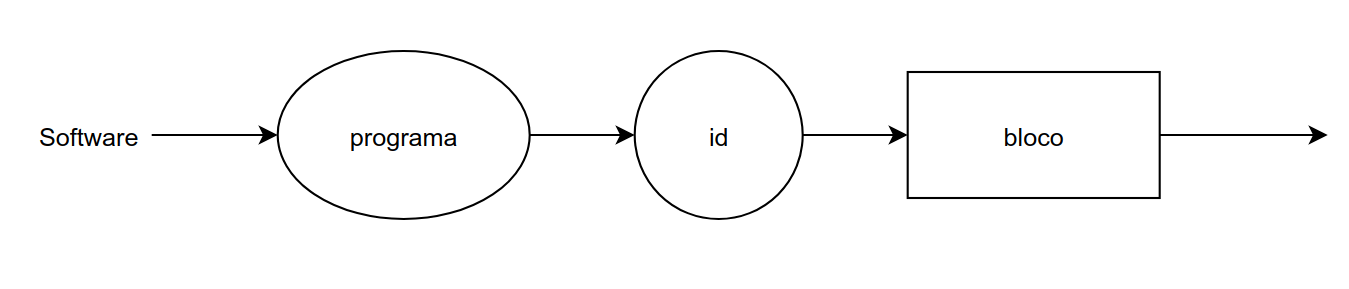
\includegraphics[]{grafos_sintaticos/software.png}
   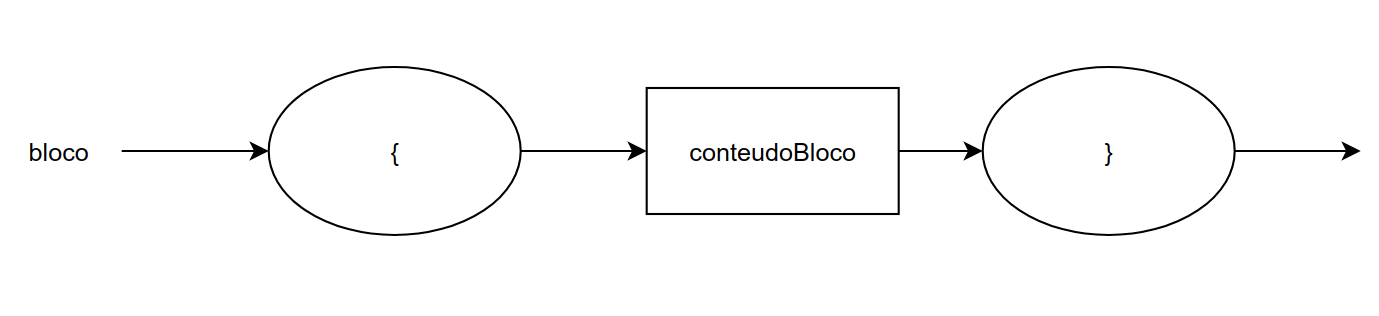
\includegraphics[]{grafos_sintaticos/bloco.png}
   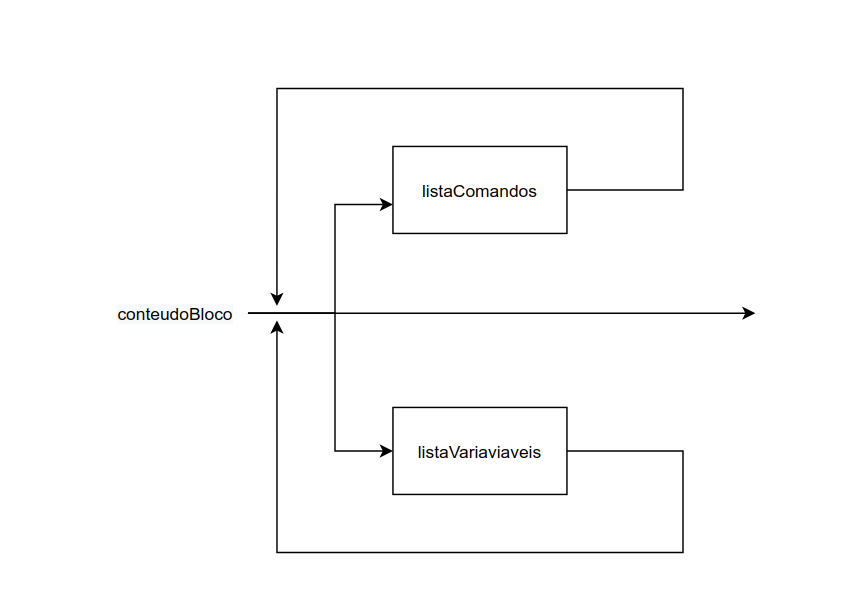
\includegraphics[]{grafos_sintaticos/conteudo_bloco.png}

   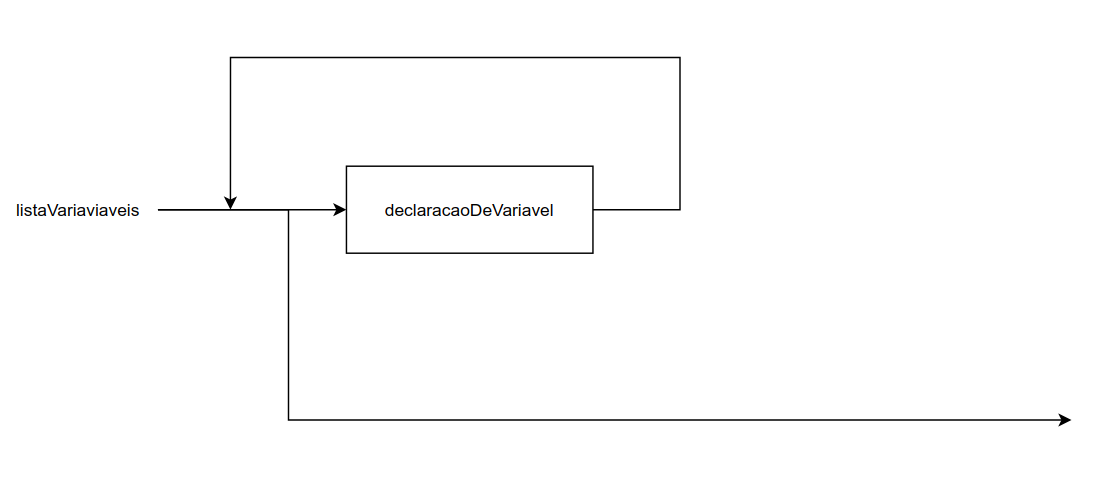
\includegraphics[]{grafos_sintaticos/lista_variaveis.png}
   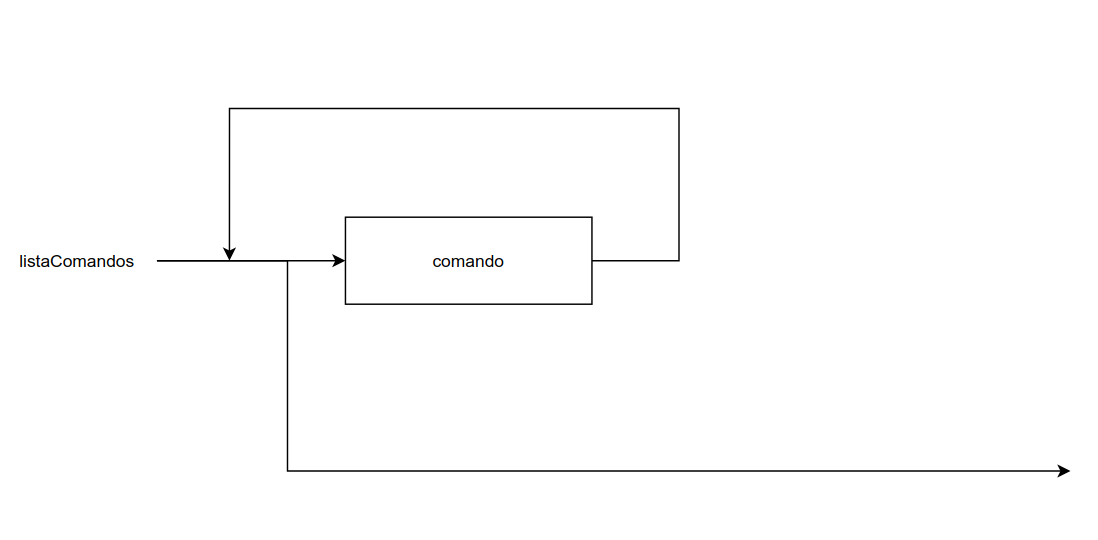
\includegraphics[]{grafos_sintaticos/lista_comandos.png}
   
\end{figure}

\newpage

\begin{figure}[H]
   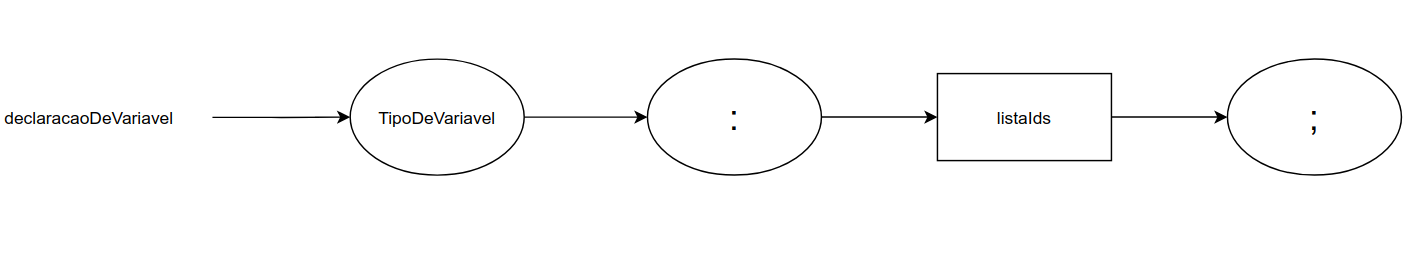
\includegraphics[]{grafos_sintaticos/declaracao_de_variavel.png}

   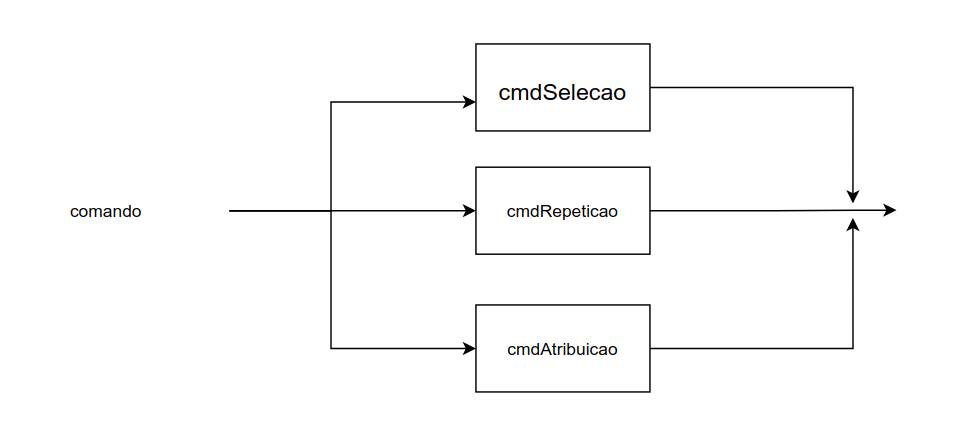
\includegraphics[]{grafos_sintaticos/comando.png}

   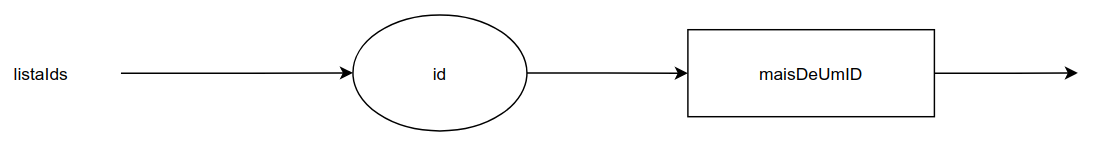
\includegraphics[]{grafos_sintaticos/lista_ids.png}

   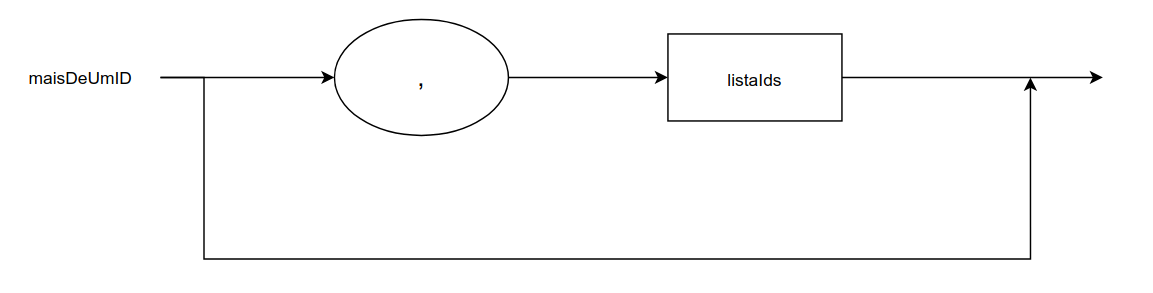
\includegraphics[]{grafos_sintaticos/mais_de_um_id.png}

   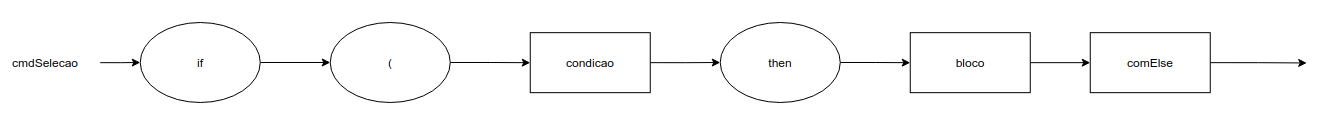
\includegraphics[scale=1.5]{grafos_sintaticos/cmd_selecao.png}



  
\end{figure}


\newpage

\begin{figure}[H]
    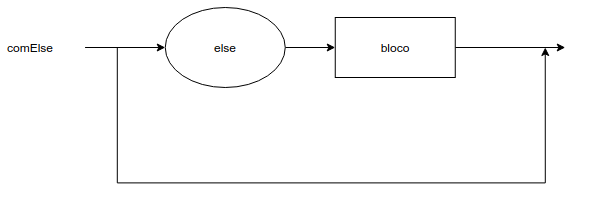
\includegraphics[scale=2.5]{grafos_sintaticos/com_else.png}

    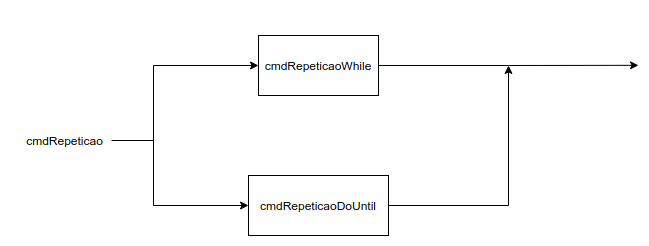
\includegraphics[scale=2.5]{grafos_sintaticos/cmd_repeticao.png}

    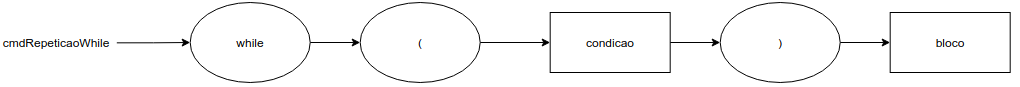
\includegraphics[scale=1.6]{grafos_sintaticos/cmd_repeticao_while.png}

    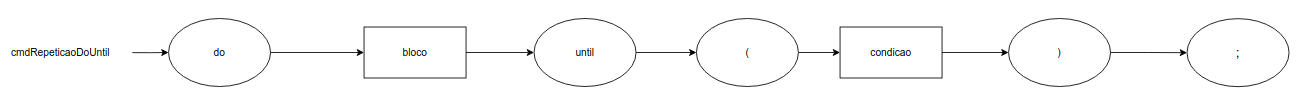
\includegraphics[scale=1.3]{grafos_sintaticos/cmd_repeticao_do_until.png}

    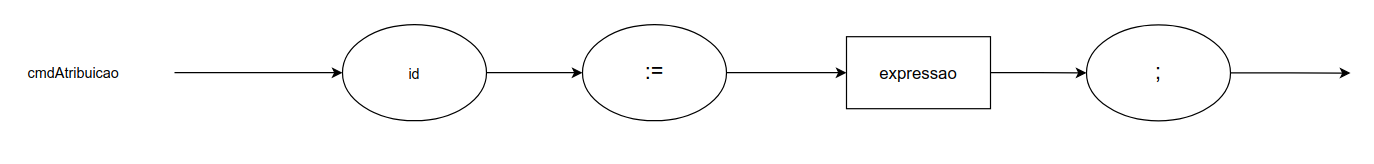
\includegraphics[scale=1.3]{grafos_sintaticos/cmd_atribuicao.png}

    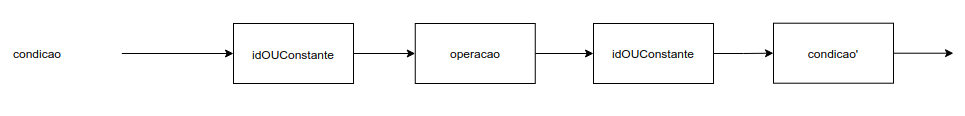
\includegraphics[scale=1.5]{grafos_sintaticos/condicao.png}

    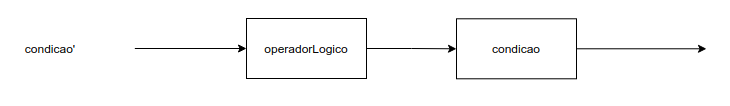
\includegraphics[scale=2.3]{grafos_sintaticos/condicao'.png}

    
\end{figure}




\newpage


\begin{figure}[H]
    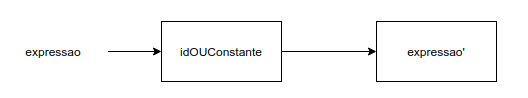
\includegraphics[scale=2.0]{grafos_sintaticos/expressao.png}

    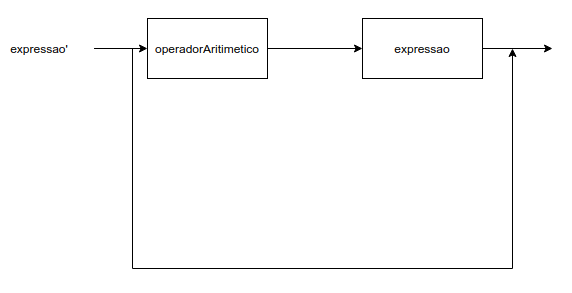
\includegraphics[scale=2.0]{grafos_sintaticos/expressao'.png}

\end{figure}

\newpage

\begin{figure}[H]
    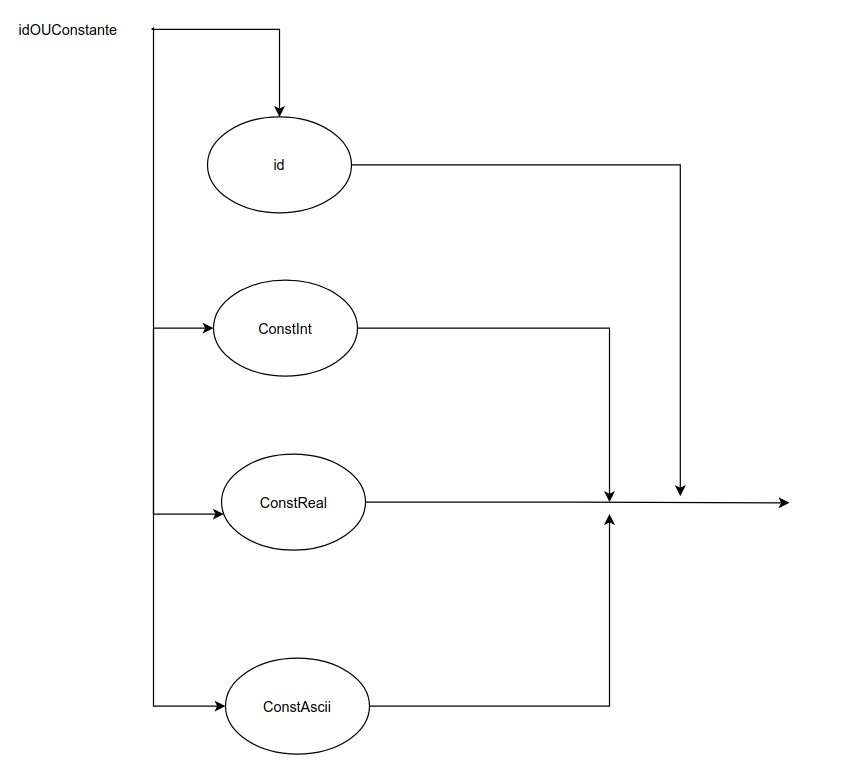
\includegraphics[scale=1.1]{grafos_sintaticos/id_ou_constante.png}

    % 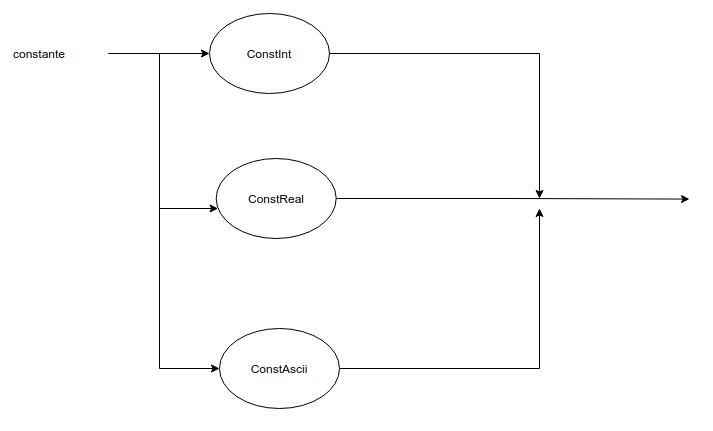
\includegraphics[scale=2.0]{grafos_sintaticos/constante.png}
\end{figure}



\end{document}